\documentclass{report}

\usepackage{polski} % Pozwala na użycie polskiego. Ustawia między innymi fontenc na T1
\usepackage[utf8]{inputenc} % Informuje o kodowaniu

\usepackage{xcolor}% http://ctan.org/pkg/xcolor
\usepackage{hyperref}% http://ctan.org/pkg/hyperref

\definecolor{LinkColor}{HTML}{1d5cc1}

\usepackage{tabto}

\usepackage{graphicx} % Pakiet do obrazów
\graphicspath{ {./Obrazy/} } % Folder, z którego będą brane obrazy

% Nie twórz nowych stron
\usepackage{etoolbox}
\makeatletter
% \patchcmd{\chapter}{\if@openright\cleardoublepage\else\clearpage\fi}{}{}{}
\makeatother

\title{Specyfikacja funkcjonalna -- Gra w życie}
\author{Krzysztof Dąbrowski i Jakub Bogusz}
\date{\today}

\begin{document}
\maketitle{}

\tableofcontents{}

\chapter{Cel projektu}
Celem projektu jest implementacja gry w życie w języku C. Gotowy program ma przeprowadzać symulację kolejnych pokoleń oraz generować na ich podstawie pliki graficzne przedstawiające etapy symulacji. Generacja odbywa się na podstawie parametrów podanych przez użytkownika w postaci flag. Program działa wyłącznie w trybie wsadowym, co oznacza, że cały proces symulacji odbywać się bez ingerencji użytkownika. Aplikacja może generować jeden z trzech rodzajów plików wyjściowych: obrazów, animacji lub plików tekstowych.

\chapter{Opis ogólny problemu}
Gra w życie jest automatem komórkowym wymyślonym przez brytyjskiego matematyka John Horton Conway
%TODO: Dopisać więcej, Czym jest siatka, czym są stany
w 1970 roku. Polega na symulacji kolejnych pokoleń życia komórek według następujących zasad.

\section{Symulacja}

\paragraph{Stany}  Komórka może znajdować się w jednym z dwóch stanów:
\begin{itemize}
\item żywa,
\item martwa.
\end{itemize}

\paragraph{Pokolenie} to stan wszystkich komórek w danej chwili. Gdy stan pokolenia jest ustalony, możliwe jest utworzenie nowego (potomnego) pokolenia komórek, powstających według poniższych zasad.

\paragraph{Reguły} Następne pokolenie generowane jest zgodnie z regułami:
\begin{itemize}
\item Jeżeli komórka była martwa i miała dokładnie 3 żywych sąsiadów, w następnym pokoleniu staje się żywa,
\item Jeżeli komórka była żywa to pozostaje żywa jeśli miała dwóch lub trzech żywych sąsiadów. W przeciwnym razie staje się martwa.
\end{itemize}

\section{Struktury}
Symulacja przeprowadzona zgodnie z powyższymi regułami może prowadzić do powstania ciekawych obiektów zwanych strukturami. 

\begin{figure}[h]
\centering
\setlength{\fboxsep}{0pt} %Odstęp 0
\setlength{\fboxrule}{1pt} %Grubość ramki 1p
\fbox{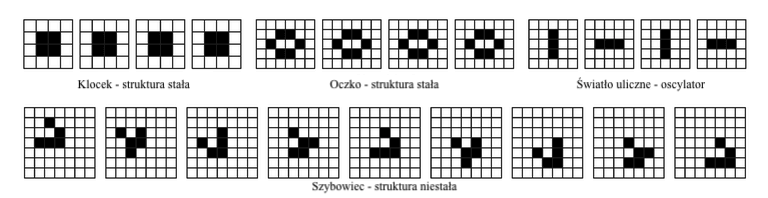
\includegraphics[width=13cm]{struktury}}
\caption{Przykłady struktur}
\end{figure}

Reguły symulacji umożliwiają również tworzenie dużo bardziej skomplikowanych struktur (jak na przykład maszyna Turinga -- https://youtu.be/My8AsV7bA94).



\chapter{Działanie programu}

\section{Komunikacja z użytkownikiem}
Program działa w trybie wsadowym. Oznacza to, że użytkownik podaje jedynie argumenty początkowe dla symulacji wraz z uruchomieniem programu (w formie flag), a następnie program automatycznie przetwarza dane i generuje wyniki.

\section{Tryb wsadowy}
\paragraph{Argumenty} \label{argumenty}
\begin{itemize}
\item \texttt{-h / --help} \\ Wyświetlenie pomocy,
\item \texttt{ -f [nazwa pliku]  / --file plik [nazwa pliku] } 
	\\ \textit{ Łańcuch znaków }będący nazwą pliku z wejściowym stanem planszy zgodny z \hyperref[format]{\textcolor{LinkColor}{formatem}}; wyklucza się z  \hyperref[s]{\textcolor{LinkColor}{flagą -s}}
\item \texttt{-o [ścieżka] / --output\textunderscore{}dest [ścieżka]}  \\\textit{ Łańcuch znaków }będący ścieżką do folderu, w którym zostaną zapisane wyniki \label{output_dest} symulacji. Domyślnie pliki  będą generowane w folderze  o nazwie będącej aktualną datą i godziną wywołania programu,
\item \texttt{-t [gif | png | txt] / --type [gif | png | txt])} \\\textit{ Łańcuch znaków }reprezentujący typ generowanych rezultatów. Domyślnie gif, \label{output_args}
\item \texttt{-n [liczba] / --number\textunderscore{}of\textunderscore{}generations [liczba]} \\ \textit{ Liczba } pokoleń do wygenerowania. Domyślnie 15,
\item \texttt{-p [liczba] / --step [liczba]} \\ \textit{ Liczba }decydująca o tym, co który stan symulacji będzie zapisywany. Domyślnie 1,
\item \label{s} \texttt{-s [LICZBAxLICZBA] / --size [LICZBAxLICZBA]} \\ \textit{ Łańcuch znaków } o formacie "XxY" (X -- szerokość planszy, Y -- wysokość planszy), będący wymiarami losowo generowanej planszy początkowej. Wyklucza się z -f, 
\item \label{delay} \texttt{-d [liczba] / --delay [liczba]} \\ Podanie tego argumentu spowoduje wyświetlanie w konsoli kolejnych pokolenie symulacji. \textit{ Liczba } ta będzie oznaczać czas  w milisekundach między wyświetleniem poszczególnych pokoleń. Wartość -1, co oznacza manualne przechodzenie do następnego pokolenia klawiszem ENTER lub zapisanie wyświetlanego pokolenia w pliku.txt wpisując ,,save''.
\end{itemize}

Wywołanie programu bez żadnego argumentu przyjmuje flagę --size 10, i wartości domyślne innych parametrów.

Wywołanie programu z błędnymi argumentami lub niewystarczającą ich liczbą wyświetli pomoc wraz z   \hyperref[przyklady]{\textcolor{LinkColor}{przykładami wywołania i ich opisami.}}

\section{Przykłady wywołania}  \label{przyklady}
\paragraph{\texttt{gra\textunderscore{}w\textunderscore{}zycie -s 5x8 -d -1}} \mbox{} \\
Program utworzy losową planszę o 5 komórkach szerokości i 8 wysokości i przeprowadzi symulację wyświetlając kolejne pokolenia w konsoli, pomiędzy którymi użytkownik będzie przełączać się wciskając ENTER oraz będzie mógł zapisać aktualnie wyświetlane pokolenie wpisując ,,save'' i zatwierdzając klawiszem ENTER.

\paragraph{\texttt{gra\textunderscore{}w\textunderscore{}zycie -f dane\textunderscore{}wejsciowe.txt -p 3 -t png -n 21}} \mbox{} \\
Program wyczyta początkową planszę z pliku o nazwie ,,dane\textunderscore{}wejsciowe.txt'', utworzy nowy folder o nazwie będącej dzisiejszą data oraz godziną i zapisze do niego 7 obrazów w formacie .png (co 3 pokolenie). 

\section{Plik wejściowy}  \label{format}
Plik wejściowy pozwala na wczytanie stanu planszy. Dzięki temu użytkownik ma kontrolę nad początkiem symulacji, oraz może kontynuować symulacje z zapisanego wcześniej etapu.

\subsection{Przykład}
5 3 \tab -- rozmiar (x y) \\
1 0 0 1 1 \tab -- Wartości poszczególnych komórek \\
0 1 1 0 1 \tab -- 1 - żywa \\
0 0 0 1 1 \tab -- 0 - martwa \\

\begin{figure}[h]
\centering
\setlength{\fboxsep}{0pt} %Odstęp 0
\setlength{\fboxrule}{1pt} %Grubość ramki 1p
\fbox{
\includegraphics[width=7cm]{Przyklad_planszy}}
\caption{Grafika wygenerowana na podstawie przykładowej planszy}
\end{figure}

\subsection{Format pliku}
\subsubsection*{Kodowanie}
Ponieważ plik powinien zawierać tylko liczby arabskie i odstępy możliwe jest dowolne kodowanie kompatybilne z ASCII. \\
\paragraph{Sugerowane kodowania to:}
ASCII, UTF-8, ISO 8859, Windows-1250

\subsubsection*{Opis formatu}
Plik w pierwszej linii powinien zawierać 2 liczby. Pierwsza z nich oznacza rozmiar planszy w poziomie, druga w pionie. \\
Następnie plik powinien zawierać tyle linii jaki został podany rozmiar w pionie. W każdej z tych linii powinno być tyle 0 lub 1 ile wynosi rozmiar w poziomie. \\
Zero oznacz komórkę martwą, a jeden komórkę żywą.

\chapter{Wyniki działania programu}
%TODO: Napisać od nowa
Wyniki działania programu będą zależeć od preferencji użytkownika -  od podanych \hyperref[argumenty]{\textcolor{LinkColor}{argumentów}}. 
\begin{itemize}
\item wyświetlić wybraną ilość pokoleń w konsoli,
\item wygenerować plik lub pliki .png z reprezentacjami graficznymi kolejnych pokoleń,
\item wygenerować plik .gif przedstawiający życie cywilizacji,
\item wygenerować plik lub pliki .txt reprezentujący konkretny stan cywilizacji, mogący służyć za plik wejściowy.
\end{itemize}

\chapter{Sytuacje wyjątkowe}
Czasem działanie programu może ulec zmianie na skutek nieprawidłowych danych wejściowych, niestandardowych ustawień wprowadzonych przez użytkownik lub z przyczyn losowych. Ten rozdział opisuje jak program zachowa się w takiej sytuacji, oraz co może ją wywołać.

\section{Zmiana domyślnego zachowania}
\paragraph{Zbyt szeroka plansza}
W przypadku gdy użytkownik włączy wyświetlanie kolejnych stanów w konsoli ale rozmiar planszy będzie zbyt szeroki by możliwe było jej wyświetlenie bez zawijania wierszy program wyświetli komunikat o niemożliwości wyświetlenia planszy w konsoli. Kolejne pokolenia nie będą wyświetlanie oknie wiersza poleceń ale generacja plików wynikowych nie ulegnie zmianie. \\
Treść komunikatu: ,,Wybrana szerokość planszy jest zbyt duża by możliwe było wyświetlenie kolejnych pokoleń w oknie konsoli.''

\section{Błędy}
Opis błędów, które mogą wystąpić w trakcie działania programu.

\subsection{Błędy pliku wejściowego}

\paragraph{Podany plik nie istnieje}
Jeśli ścieżka podana przez użytkownika jest błędna program wyświetli komunikat o braku możliwości otwarcia wskazanego pliku i zakończy pracę. \\
Treść komunikatu: ,,Nie udało się otworzyć wskazanego pliku.''

\paragraph{Pusty plik}
W przypadku gdy plik wskazany przez użytkownika będzie pusty program powiadomi o tym i zakończy pracę. \\
Treść komunikatu: ,,Wskazany plik wejściowy jest pusty.''

\paragraph{Rozmiar planszy nie będący liczbą}
Jeśli w pierwszej lini pliku znajdować się będą wartości inne niż liczby program nie będzie w stanie wczytać rozmiaru planszy. W takiej sytuacji wyświetli odpowiedni komunikat i zakończy pracę. \\
 Treść komunikatu: ,,Nie udało się wczytać rozmiaru planszy.''
 
 \paragraph{Niedodatni rozmiar planszy}
 Jeśli jeden z wymiarów planszy nie będzie dodatnią liczbą całkowitą program zasygnalizuje błąd i zakończy pracę. \\
 Przykładowy komunikat: ,,Szerokość musi być większa od 0. Podana szerokość to -5.''
 
 \paragraph{Brak nowej linii po rozmiarze planszy}
 W przypadku gdy po wysokości planszy w pliku będzie inny znak niż przejście do nowej lini program zasygnalizuje błąd i zakończy pracę. \\
 Treść komunikatu: ,,Spodziewany koniec lini po wymiarze planszy.''
 
 \paragraph{Błąd przy wczytywaniu stanu komórki}
 Jeśli nie uda się wczytać stanu komórki, na przykład ponieważ w pliku jest za mało linii lub jedna z linii jest zbyt krótka, program wypisze, w którym miejscu pliku wystąpił błąd i zakończy pracę. \\
 Przykładowy komunikat: ,,Wystąpił błąd przy próbie przeczytania znaku w lini: 3 kolumnie: 8.''
 
 \paragraph{Nieprawidłowy znak w pliku}
 Jeśli podczas czytania pliku program napotka nieprawidłowy znak wypisze na jakiej pozycji w pliku napotkany został nieprawidłowy znak, jaki to znak, oraz czego spodziewał się program. \\
 Przykładowy komunikat: ,,Niewspierany znak napotkany w lini: 2 kolumnie: 1. Spodziewana wartość: 0 lub 1. Napotkana wartość: T''

\subsection{Błędy losowe}
\paragraph{Brak pamięci operacyjnej}
Gdyby w systemie zabrakło pamięci program nie będzie w stanie funkcjonować poprawnie. Program wyświetli komunikat o błędzie i przerwie pracę. \\
Treść komunikatu: ,,Program nie uzyskał pamięci od systemu operacyjnego. Spróbuj uruchomić program ponownie za pewien czas.''

\end{document}
